\documentclass[a4paper,11pt]{report}
%\usepackage{hyperref}
\usepackage{url,natbib,amssymb,hyperref,graphicx,wrapfig,setspace,multirow,booktabs,subfig,array,wrapfig,calc}
\usepackage{array}
\newcolumntype{P}[1]{>{\centering\arraybackslash}p{#1}}
\usepackage{fancyhdr}
\usepackage{color}
\usepackage{booktabs,caption,fixltx2e}
\usepackage[round]{natbib}      % References with names and years
\usepackage{xr}                 % reference anothe chapter
%\externaldocument[2-]{../CHAPTER2/ch2_LSM_v11}
%\externaldocument[3-]{../CHAPTER3/ch3_sensitivity_v10}
\usepackage{graphicx}
\usepackage{caption}
\usepackage{appendix}
%\usepackage{subfigure}
\usepackage{float}
\usepackage{subfig}
\usepackage{float}
\usepackage{paralist}                % inline lists
\usepackage{gensymb}    % degrees celsius as {\celsius}
%\usepackage{textcomp]    % arrows
\newcommand{\tildetext}{\raise.17ex\hbox{$\scriptstyle\mattt{\sim}$}}
\usepackage{rotating}   %rotate table
%\renewcommand{\arraystretch}{1.5}  %increase space between rows in tables (default is 1) because there is already baselinestrech 1.5 tables become too separated, maybe with normal spacing this command should be used
\usepackage{rotating,booktabs}
\usepackage{threeparttable}
\usepackage{multirow}
\usepackage{color}% color the text
\usepackage{amsmath}
% Page setup from thesis template
\topmargin=-10mm
\textwidth=150mm
\textheight=234mm
\headsep=12mm
\oddsidemargin=14mm
%\oddsidemargin=12mm
\evensidemargin=-1mm
%\evensidemargin=1mm
\parindent=6mm
\parskip=1em 

\newlength{\rulewidth}
\setlength{\rulewidth}{150mm} % change to 150mm for printing on
			      % gordon, 149 otherwise???
% 1.5 line spacing so my supervisor can scrawl all over it
\renewcommand{\baselinestretch}{1.50}

\pagestyle{headings}    % chapter number on top

\setcounter{secnumdepth}{4}              %Numbers subsubsections, and lower.
\setcounter{tocdepth}{4}                 %Sets depth of table of contents to include subsubsections.

\pagestyle{fancy}
\fancyhf{}
%\rhead{\fancyplain{}{\textit{\nouppercase\rightmark}}}
\fancyhead[L]{Chapter 3. Models and methods}
\fancyfoot[C]{ \thepage\ }

%opening
\title{}
\author{Renato Kerches Braghiere \\ This document was written in \LaTeX \\ Number of words: 18135}
\date{\today}

\begin{document}
\maketitle
\setcounter{chapter}{2} %so next one is 3

\chapter{Models and methods}

\section{Introduction}\label{introduction}

In here comes a brief introduction

\section{Radiative transfer models}\label{section:RTMs}

\subsection{The Two-stream scheme} 
The Two-Stream scheme assumes that diffuse radiative fluxes are isotropic in the upward and downward directions. Supposing that the upper and lower leaf optical properties are identical, the Two-Stream scheme used to model radiative transfer in plant canopies is given in the following form \citep{Dickinson1983,Sellers1985}: 
\begin{equation}
\begin{gathered}
-\overline{\mu}(dI^{\uparrow})/dL + [1 - (1 - \beta)\omega]I^{\uparrow} - \omega \beta I^{\downarrow} = \omega \overline{\mu} K \beta_0 \exp{(-KL)},\\
-\overline{\mu}(dI^{\downarrow})/dL + [1 - (1 - \beta)\omega]I^{\downarrow} - \omega \beta I^{\uparrow} = \omega \overline{\mu} K (1-\beta_0) \exp{(-KL)}
\end{gathered}
\label{equation:ts}
\end{equation}
\noindent where $I^{\uparrow}$ and $I^{\downarrow}$ are the upward and downward diffuse radiative fluxes normalized by the incident flux respectively, $\mu$ is the cosine of the zenith angle of the incident beam, $K$ is the optical depth of direct beam per unit leaf area and is equal to $G(\mu)/\mu$, $G(\mu)$ is the relative projected area of leaf elements in the direction $cos^{-1}\mu$, $\overline{\mu}$ is the average inverse diffuse optical depth per unit leaf area and is equal to $\int_{0}^{1}[\mu^{\prime}/G(\mu^{\prime})]d\mu^{\prime}$, $\mu^{\prime}$ is the direction of scattered flux, $\omega$ is the scattering coefficient and is equal to $\rho_{leaf} + \tau_{leaf}$, and $L$ is the cumulative LAI. $\beta$ and $\beta_0$ are upscattering parameters for the diffuse and direct beams respectively (see \citet{Sellers1985} for details). 

The version used in this exercise was extracted from the JULES model. The JULES model is the UK community land surface model designed to be interfaced with the UK Met Office Unified Model \citep{Walters2014} by predicting fluxes of heat, water and carbon between the land surface and the atmosphere. It originates from the Met Office Surface Exchange Scheme (MOSES) \citep{Cox1999}, and it includes the TRIFFID (Top-down Representation of Interactive Foliage and Flora Including Dynamics) dynamic vegetation model \citep{Cox2001}. The physical basis of JULES is common to most of the land surface models and are described in details in \citet{Best2011} and \citet{Clark2011}.

JULES uses a number of layers (10 in this exercise) with equally distributed LAI to calculate the radiative transfer in the canopy for direct and diffuse radiation separately. The leaves extinction properties are prescribed by leaf reflectance ($\rho_{leaf}$) and transmittance ($\tau_{leaf}$) in the PAR and NIR wavebands and canopy leaf angle distribution (spherical or horizontal). The amount of absorbed incident radiation at each layer is therefore determined by sun zenith angle, incident direct and diffuse radiation at the top of the canopy, and the leaves extinction coefficients.

\subsubsection{Canopy radiative transfer option 4}

\subsubsection{Canopy radiative transfer option 5}

\section{Handling vegetation heterogeneity in LSMs}
Full 3D radiative transfer models require a large number of parameters, and a high computational demand, thus, 1D radiative transfer approaches are still preferably used \citep{yang2003,loew2014}. However, more simplified approaches to handle sparse vegetated canopies have been implemented in LSMs, and are widely used \citep{loew2014}. The vegetation cover approach divides one grid cell in a number of tiles, where each tile has its own characteristics. The possible number of tiles and their parameters depend on each LSMs.

Suppose a model grid cell with area $A$, which is assumed to be fully covered (100\%) by a particular vegetation type. In the case of sparser canopies, e.g. savannahs, the area $A$ is covered by a dominant vegetation type, usually taller trees, but often presents a second vegetation type, for example, understory vegetation (e.g. shrubs, grass) and so on, or part of the grid with no vegetation at all is covered by bare soil. The total area $A$ is thus defined as,
\begin{equation}
A = f_{veg} + f_{under}
\label{equation:area}
\end{equation}
\noindent where $f_{veg}$ is the fractional coverage of the major vegetation type and $f_{under}$ can correspond to a different vegetation type or the soil surface.
In this case $f_{under}$ is equivalent to the between-crown gaps. The total direct transmissivity, or the gap probability with Sun above head ($\theta$ = 0$^{\circ}$) is always greater than or equals to $f_{under}$. Figure~\ref{f:loew2014} from \citet{loew2014} shows a representation of a sparse vegetation canopy with $f_{veg}$ being the percentage of the area covered by a single vegetation type, $f_{under}$ is the remaining area, and P$_{gap}$($\theta$=0$^{\circ}$) as being $f_{under}$ plus the within-crown gap probability.

\begin{figure}
\centering
\includegraphics[width=0.5\textwidth]{/home/mn811042/Thesis/chapter4/figures/Sec_4.2/figure1_pgap_fveg_funder_loew.png}
\caption{Illustration of the difference between vegetation fraction ($f_{veg}$) and gap probability (P$_{gap}$($\theta$ = 0)) for a model grid cell (extracted from \citet{loew2014}).} 
\label{f:loew2014}
\end{figure}

The canopy radiative transfer scheme in most LSMs (e.g. JULES \citep{Clark2011}, CLM \citep{Bonan2002}, NOAH \citep{Niu2011}, etc)  is based on the two-stream scheme \citep{sellers1985} which calculates surface albedo and canopy absorption. In JULES, the total fAPAR of a grid cell is calculated by simply weighting the fAPAR calculated by the radiative transfer scheme by the actual area covered by vegetation as, 
\begin{equation}
fAPAR = f_{veg} \cdot fAPAR_{canopy}
\label{equation:faparvegfraction}
\end{equation}
And the correspondent surface albedo ($\alpha$) can be obtained as, 
\begin{equation}
\alpha = f_{veg} \cdot \alpha_{canopy}  +  f_{under} \cdot \alpha_{soil}
\label{equation:albedovegfraction}
\end{equation}
\noindent where $\alpha_{soil}$ is the soil albedo. The solar spectrum bands in JULES are determined by the spectral properties of leaves and soil.

In this section the tile fraction correction as done in JULES and other LSMs (reference) is applied to the same canopies described in the previous section. It is important to note that the tile fraction correction affects not only the radiative transfer in LSMs, but other parts of the model related to water and carbon balances as well. Here, the impacts of this correction is evaluated over the radiative components of the radiation partitioning in the model in two shortwave wavebands, PAR and NIR.

Table~\ref{tab:fveg} shows the vegetation fraction ($f_{veg}$) and the gap probability with Sun above head (P$_{gap}$($\theta$=0$^{\circ}$)) for the three evaluated canopy structures with same LAI. 

\subsection{Tree-based model: MAESPA}\label{section:maespa}
The MAESTRA/MAESPA model \citep{Wang1990,Medlyn2004,Medlyn2007,Duursma2012} represents a forest canopy as an array of tree crowns, whose positions and dimensions are specified. The radiation routines are described in detail by \citet{Wang1990}. The canopy consists of individual tree crowns, which are described by a basic shape (one of several shapes, including ellipsoids, cylinders and cones), length, height to crown base, and width (in x and y directions). Radiation calculations are performed only for a set of target crowns specified by the user. The distribution of leaf area within the target crown is specified, as is the leaf angle distribution. The target crown is divided into usually 60 grid points, and the radiation penetrating to each grid point is calculated for three wavebands (PAR, NIR and thermal infra-red, TIR) based on shading within the crown, shading by neighbouring trees, the location of the sun, and whether radiation is direct or diffuse. Direct, diffuse and scattered radiation are considered separately. Scattering of radiation is approximated following \citet{Norman1979}. Leaf area within crowns is assumed to be distributed randomly \citep{Wang1990}. At each grid point, leaf area is separated into sunlit and shaded leaf area (Norman, 1993). The model has previously been applied to study canopy carbon and water fluxes of \textit{Picea sitchensis} \citep{Wang1990}, \textit{Pinus radiata} \citep{McMurtrie1993}, \textit{Betula pendula} \citep{Wang1998}, and \textit{Pinus taeda} \citep{Luo2001}. 
%Using the $R$ (R Development Core Team, 2011) package, Maeswrap (Duursma, 2015), the 3D stand scenes were graphically reproduced in 3D.

\subsection{Geometric optics model: GORT}\label{section:gort}
The GORT model was developed to describe the effects of three-dimensional canopy structure on the radiation environment and to characterise the heterogeneous radiation environment in natural vegetation at the forest stand scale \citep{Li1995}. Merging theory from geometric optics and radiative transfer, the GORT model treats vegetation canopies as assemblages of randomly distributed tree crowns of ellipsoidal shape. The tree crowns are filled with leaves that absorb and scatter radiation passing through the crown. Principles of radiative transfer are used in describing the multiple scattering of leaves inside crowns and the multiple scattering among crowns and the ground surface. The GORT model was extended by \citet{Ni1997} to include the vertical canopy gap probability profile. For this exercise the PAR radiation spectrum was centred in 550 nm, and NIR in 850 nm.

\subsection{Monte-Carlo model: raytran}\label{section:raytran}

The RAMI4PILPS \citep{Widlowski2011} suite of experiments was designed to evaluate the accuracy and consistency of shortwave radiative transfer formulations as used in GCMs by evaluating different models against the extensively verified 3D reference Monte Carlo ray-tracing model, known as raytran \citep{Govaerts1995}.

One of the specificities of the RAMI4PILPS suite ofexperiments is that model simulations can be compared against a reference data set of relatively well known uncertainty. The latter was provided by the 3‐ D MonteCarlo ray‐tracin g m odel kn own as raytran [Govaerts andVerstraete, 1998]. The raytran model has been comparedextensively against goniometer measurements [ Govaerts,1995], field observations [Widlowski et al., 2005a] and,more systematically, against other RT models in the contextof the RAMI activity [Pinty et al., 2001, 2004b; Widlowskiet al., 2007]. Due to its excellent performance with respectto energy conservation, and its matching of analytical solu-tions to within 10−4on average, the raytran model wasidentified as one of six credible 3‐ D canopy RT models andchosen to contribute to the development of a reference dataset against which other radiative transfer models could thenbe evaluated. This reference data set is based on the RAMIsimulations of all six credible 3‐D Monte Carlo models(having a mutual divergence of less than 1% over manythousands of model runs) and has become the cornerstoneof the RAMI On‐line Model Checker (http://romc.jrc.ec.europa.eu/) a web ‐based facility for the autonomousbenchmarking of canopy reflectance models [Widlowski et al.,2008].

The ray-tracing code used in the RAMI4PILPS experiment allows the explicit representation of radiation transfer in arbitrarily complex scenes \citep{Govaerts1998} by implementing a Monte Carlo approach where the fate of millions of individual rays are followed as they travel through the computer simulated scene. This model implements the most detailed and most faithful simulations of radiation transfer, but as other complex models is rather expensive computationally. 

In this thesis, the RAMI4PILPS heterogeneous canopy scenario, referred as ``Open Forest Canopy'' was used, where tree crowns were approximated by woodless spheres in an open forest canopy scene. Details of the RAMI4PILPS experiments used in this present study are summarised in Table~\ref{tab:RAMI4PILPS} and a graphic representation of the experiment setups can be found in Fig.~\ref{fig:rami}, while further details of the RAMI4PILPS experiments can be found in \citet{Widlowski2011}. 

For each scenario, simulations for different leaf area index and varying soil brightness are performed, assuming direct insulation for three different sun zenith angles, as well as isotropic illumination conditions, i.e. global incident radiation is totally diffuse.

In a first analysis, the participant parameterisations (see section~\ref{section:parameterisations}) were compared in two different ways:
\begin{enumerate}[i]
\item by evaluating the behaviour of the structural indices (clumping indices and structure factor) varying with Sun zenith angle, and
\item by comparing the direct transmissivity ($P_{gap}(\theta)$) calculated with Eq.~\ref{equation:pgap} for each one of the different `structural indices'.
\end{enumerate}

\begin{threeparttable}
\centering
\caption{Summary of variables defining structurally heterogeneous scenes (see \citet{Widlowski2011} for details). Different soil albedos are defined as BLK = black, MED = medium, SNW = snow.}
%\begin{tabular*}{\textwidth}{ l@{\extracolsep{\fill}}*{4}{c}}
\begin{tabular}{l{0.25\textwidth} l{0.75\textwidth}}
%\begin{tabular}{\textwidth}{|p{\textwidth/4}|p{\textwidth/4}|p{\textwidth/4}|p{\textwidth/4}|}
%\begin{tabular*}
     \hline
     \hline
\textbf{Variable Identification}   & \textbf{Values (Units)}\\
\noalign{\smallskip}\hline
Leaf Area Index/ canopy	                & 0.50$^S$, 1.50$^M$ and 2.50$^D$ (m$^2$.m$^{-2}$)\\
Leaf Area Index/ sphere	                & 5.0$^S$, 5.0$^M$ and 5.0$^D$  (m$^2$.m$^{-2}$)\\
1 - $P_{gap} (\theta = 0^{\circ})$      & 0.09$^S$, 0.26$^M$ and 0.434$^D$\\
Tree density                            & 12.80$^S$, 38.24$^M$ and 63.68$^D$ (trees/hectare)\\
Maximum canopy height                   & 16 m\\
Minimum sphere centre height	        & 7 m\\
Maximum sphere centre height	        & 11 m\\
$\alpha_{soil}$,PAR / $\alpha_{soil}$,NIR	& BLK: 0.00/0.00; MED: 0.12/0.21; SNW: 0.96/0.56\\
Soil scattering law	                & Lambertian\\
$\rho_{leaf}$,PAR / $\rho_{leaf}$,NIR     & 0.0735/0.3912\\
$\tau_{leaf}$,PAR / $\tau_{leaf}$,NIR     & 0.0566/0.4146\\
Leaf scattering law                     & Bi-Lambertian\\
Sun zenith angle	                & 27.5$^{\circ}$/60.0$^{\circ}$/83.5$^{\circ}$/Isotropic(ISO)\\
Scatterer Normal Distribution           & Spherical\\
Woody area index                        & 0.0 (m$^2$.m$^{-2}$)\\
\hline
\hline%\noalign{\bigskip}
%\end{tabular*}
\end{tabular}
\begin{tablenotes}
      \small
      \item $^S$Sparse vegetation. $^M$Medium vegetation. $^D$Dense vegetation. 
\end{tablenotes}
\label{tab:RAMI4PILPS}
\end{threeparttable}
\bigskip

\begin{figure}
\centering
\begin{tabular}{lll}
\subfloat[Sparse Canopy]{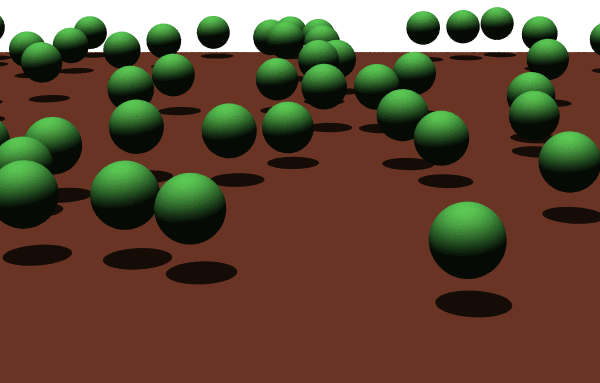
\includegraphics[width=0.33\textwidth]{/home/mn811042/Thesis/chapter4/figures/rami_lai_050.png}}
\subfloat[Medium Canopy]{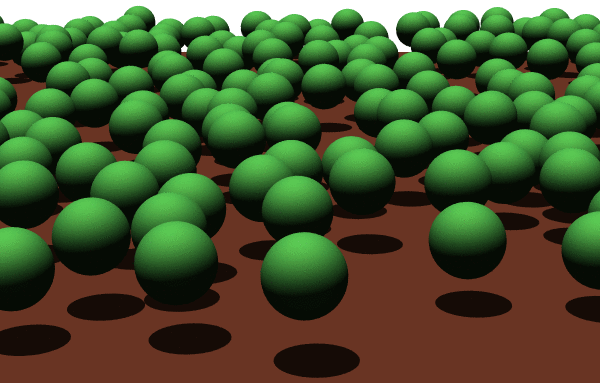
\includegraphics[width=0.33\textwidth]{/home/mn811042/Thesis/chapter4/figures/rami_lai_150.png}}
\subfloat[Dense Canopy]{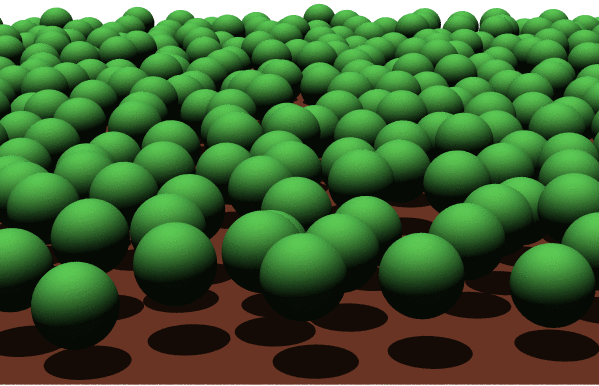
\includegraphics[width=0.33\textwidth]{/home/mn811042/Thesis/chapter4/figures/rami_lai_250.png}}
\end{tabular}
\caption{Graphical representation of the open forest canopy environments used in RAMI4PILPS. The images represent three different canopy structures \citep{Widlowski2011}.} 
\label{fig:rami}
\end{figure}

\section{The Two-stream scheme with clumping: parameterisation schemes}\label{section:parameterisations}

Several previous studies have suggested with observations and detailed modelling approaches that vegetation 3D structure influences radiation partitioning and other land surface related processes \citep{Nilson1971,Wang1990,Chen1996,Kucharik1999,Yang2001,yang2003,Jonckheere2004,pinty2006,Chen2008,Ni-Meister2010,Widlowski2011,Kobayashi2012,Loew2014}.

For most natural woody vegetation such as conifers and savannahs, the spatial distribution of individual tree crowns creates clear spaces where beam radiation propagates without interference of vegetation elements, and because of that the two-stream scheme results in large deviations from the actual amounts of absorbed and reflected radiation \citep{Ni-Meister2010,Kobayashi2012,Loew2014}.

For detailed computation of 3D radiation fields within complex vegetation canopies, radiative transfer schemes can use a geometrical optical approach and treat mixtures of individual trees and multiple scattering with foliage clumped within tree crowns, e.g. in the GORT model \citep{Li1995}. Another approach is to treat it heterogeneously between tree crowns, e.g. in MAESTRA/MAESPA \citep{Wang1990,Duursma2012}, among others more complex approaches. However, these models cannot be directly used in GCMs due to their extreme computational power demand \citep{Yang2001} and the high number of required vegetation structural parameters \citep{Loew2014}. 

Even though efficient 1D radiative transfer schemes are still preferably used, because of their simplicity, speed and suitability to run over large areas, the use of effective radiative state variables to express the properties of 3D vegetation canopy systems makes a simpler model to analogously simulate the radiation balance of more complex 3D models \citep{Pinty2004,pinty2006}, hereafter clumping schemes.

Thus the clumping schemes  account for all phyto and woody elements composing the vegetation canopy, and when its value is greater than 1, it is an indication of specific structural canopy conditions associated with significant amounts of woody elements \citep{pinty2006}. 

The first proposed `clumping index' \citep{Nilson1971,Norman1974,chen1992,Chen1996} is associated with the heterogeneous nature of the canopy volume, often used at the tree resolution, and revisited later on by other authors \citep{Pinty2004,pinty2006}, who used the same scientific proposition to account for structural heterogeneity of different radiative media at stand scale, specially in association with satellite products.

Few other authors \citep{Kucharik1999,pinty2006,Ni-Meister2010} attempted to formulate simplified modelling approaches to resolve vegetation clumping at several levels of organisation, in order to address the major differences in shortwave radiation partitioning between 1D and 3D radiative transfer schemes over non-homogeneous forest canopies all over the world.

The next sections will describe and evaluate 3 different clumping schemes to address vegetation heterogeneity in the modified two-stream scheme. Evaluations will be performed against a benchmarking exercise of radiation transfer in vegetation canopies, the RAMI4PILPS experiment \citep{Widlowski2011}.

\subsection{Adapting the two-stream scheme}

The clumping index ($\zeta(\mu)$) is introduced into the two-stream scheme by modifying three main groups of variables to account for canopy structural effects:

\begin{enumerate}
\item the optical depth of direct beam per unit leaf area, $K$; 
\item the average inverse diffuse optical depth per unit leaf area, $\mu$̅; and, 
\item the single scattering albedo, $a_s(\mu)$, used to obtain the upscattering parameters for the diffuse and direct beams, $\beta$ and $\beta_0$.
\end{enumerate}

The structure factor can be included on the optical depth of direct beam per unit leaf area, by modifying $K$ as:
\begin{equation}
K_{Struc}(\theta) = \frac{G(\theta)}{\mu} \cdot  \zeta(\mu)
\label{equation:opticaldepthstruct}
\end{equation}

The same analogy can be applied when calculating the average inverse diffuse optical depth per unit leaf area, $\bar{\mu}$, but obtaining the structure factor for the direction of scattered flux, $\mu^\prime$:
\begin{equation}
\overline{\mu_{Struc}} = \int_{0}^{1} \frac{\mu^\prime}{G(\mu^\prime) \cdot \zeta(\mu^\prime)} d\mu^\prime
\label{equation:muprimestruct}
\end{equation}

The parameter $\omega\beta$ can be inferred from the analysis of \citet{Norman1975} in the case of a single leaf whose normal is oriented at zenith angle $\theta_l$ from the local vertical defined in the upward hemisphere:
\begin{equation}
\omega\beta = \frac{1}{2}(\omega_l + \delta_l \cos^2 \theta_l)
\label{equation:omegabeta}
\end{equation}
\noindent where $\omega_l = \rho_{leaf} + \tau_{leaf}$ and $\delta_l = \rho_{leaf} - \tau_{leaf}$. 

The equation~\ref{equation:omegabeta} however is only valid for a single leaf and to obtain the total contribution of leaves over the canopy it is necessary to integrate over the appropriate leaf orientation probability distribution, between 0 and $\pi/2$, because the leaf normal are assumed to be oriented into the upward hemisphere, as in:
\begin{equation}
\omega\beta = \frac{1}{2}\Big(\omega_l + \delta_l \int_{0}^{\pi/2} \cos^2 \theta_l g^\prime(\theta_l) \sin \theta_l d\theta_l\Big)
\label{equation:omegabeta2}
\end{equation}
\noindent where $\sin\theta_l$ is introduced for normalisation requirement of the probability distribution function. And when isolating $\beta$, it is possible to obtain the generic diffuse upscatter parameter:
\begin{equation}
\beta = \frac{1}{2\omega}\Big(\omega_l + \delta_l \int_{0}^{\pi/2} \cos^2 \theta_l g^\prime(\theta_l) \sin \theta_l d\theta_l\Big)
\label{equation:beta}
\end{equation}

If the two-stream scheme equations are solved when $\omega \rightarrow 0$, i.e., single scatter approximation and semi-infinite canopy, the upward diffuse flux at the top of the canopy may be taken as equal to the single scattering albedo ($a_s(\mu)$). The equation for the direct upscatter parameter, $\beta_0$, is
\begin{equation}
\beta_0 = \frac{1 + \overline{\mu}K}{\omega\overline{\mu}K}a_s(\mu)
\label{equation:betazero}
\end{equation}

And $a_s(\mu)$ is given by, 
\begin{equation}
a_s(\mu) = \frac{\omega}{2}\int_{0}^{1} \frac{\mu^\prime G(\mu)}{\mu G(\mu^\prime) + \mu^\prime G(\mu)} d\mu^\prime
\label{equation:alphas}
\end{equation}

The equation above is only valid when assuming isotropic scattering for the leaf elements, which makes the scattering phase function independent of the angle of the incident beam (see \citet{Dickinson1983} and \citet{Sellers1985} for more details). 

The addition of the structure factor into the single scattering albedo formulation results in,
\begin{equation}
a_s(\mu) = \frac{\omega}{2}\int_{0}^{1} \frac{\mu^\prime G(\mu) \zeta(\mu)}{\mu G(\mu^\prime) \zeta(\mu^\prime) + \mu^\prime G(\mu)\zeta(\mu)} d\mu^\prime
\label{equation:alphasstruct}
\end{equation}

In this case the formulation for the direct upscatter parameter considering canopy structure is: 
\begin{equation}
\beta_0 = \frac{1 + \overline{\mu_{Struc}}K_{Struc}}{\omega\overline{\mu_{Struc}}K_{Struc}}
\bigg[\frac{\omega}{2}\int_{0}^{1} \frac{\mu^\prime G(\mu) \zeta(\mu)}{\mu G(\mu^\prime) \zeta(\mu^\prime) + \mu^\prime G(\mu)\zeta(\mu)} d\mu^\prime \bigg]
\label{equation:alphasstruct}
\end{equation}

\subsection{The clumping index by Kucharik et al. (1999)}
The parameterisation described in this subsection was developed by \citet{Kucharik1999}. The authors used measurements of LAI and gap fraction made with MVI (Multiband Vegetation Imager) \citep{Kucharik1997} obtained during the BOREAS (Boreal Ecosystem-Atmosphere Study) \citep{Sellers1997} field campaigns of 1994-1996 to derive a semi-empirical relationship between $\Omega(\theta)$ and solar zenith angle ($\theta$). 

In this method, two key quantities are needed: (i) the fraction of ground area covered by the horizontal projection of crown envelopes ($f_c$) (from nadir view), which is a function of the typical tree crown diameter ($D$), and tree stem spacing ($\lambda$), or stem density, within a study plot; and (ii) an estimate of crown porosity ($\Phi$); this quantity is related to foliage density and defined as the gap fraction within crown envelopes divided by $f_c$.
 
A series of zenith gap fraction measurements were needed along a transect beneath a canopy to partition the total gap fraction ($f_{gap},t(0)$) between within-crown and between-crown gaps, and  an estimate of the total fraction of ground area covered by the horizontal projection of crown envelopes ($f_c$). To obtain $f_c$, the typical crown silhouette area ($\pi R^2$, where $R$ is the crown radius in the horizontal direction) is multiplied by the number of crowns and divided by the total ground unit area on which the stem density is based. If $f_c$ is greater than 1, crowns typically overlap in the forest, and the entire value of $f_{gap},t(0)$ can be defined as within-crown gap fraction ($f_{gap},c(0)$). The total gap fraction occurring between-crowns ($f_{gap},b(0)$) can be estimated by $1 - f_c$, and $f_{gap},c(0)$ is therefore approximated by $f_{gap},t(0) - f_{gap},b(0)$. If the value of $f_{gap},c(0) < 0$, it can be assigned a value of 0 for all practical purposes. 

Crown porosity ($\Phi$) is determined by dividing $f_{gap},c(0)$ by $f_c$ ($\Phi$ = $f_{gap},c(0)/f_c$). The value of $\Phi$ may be described as a normalised within-crown gap fraction. Generally, an error of about 0.05 exists in determining $f_c$ and $\Phi$ by using an average crown radius and tree stem density rather than the actual model calculations of $f_c$. However, the authors indicated that these errors are not of concern when estimating $\Omega(0)$ using the gap-fraction partitioning strategy.

Values of $\Phi$ and $f_c$ were then used to determine a value of $\Omega$(0) that was consistent with calculations resulting from numerical simulations of the canopy gap-size distribution. A non-linear least-squares fit to approximately 250 Monte Carlo simulations (analysing values of $\Omega(0)$) was performed for values of $f_c$ $\geq$ 0.20, and for all simulated values of $\Phi$. A separate fit to the entire set of model data was performed for 0.04 $\geq f_c \geq$ 0.30. For sparse canopies where $f_c < 0.20$, a value of $\Omega(0)$ could still be determined. 

Ten equations were solved simultaneously to determine 10 coefficients ($a_0$, ..., $a_9$) that describe the relationship between values of $\Omega(0)$, $f_c$, and $\Phi$. To characterise the angular dependence of $\Omega(\theta)$, a minimum value of $\Omega(\theta)$ was determined at $\theta$ = 0$^{\circ}$ and a value of $\Omega(\theta)$ was needed at $\theta$ = 90$^{\circ}$. Because it was assumed that $\Omega(\theta)$ reaches its maximum value at $\theta$ = 90$^{\circ}$, \citet{Kucharik1999} refer to this value as the maximum possible element clumping index, $\Omega_{max}$, and defines it as:
\begin{equation}
\Omega_{max} = \Big(\frac{ND}{\sqrt{A}}\Big)^{0.7}
\label{equation:clumpmax}
\end{equation}
\noindent where $N$ is number of stems within ground area $A$, and $D$ is crown diameter. If $ND/\sqrt{A} > 1$, then the value of $\Omega_{max} = 1$. The angular dependence of $\Omega(\theta)$ was defined by \citet{Kucharik1999} following the equation: 
\begin{equation}
\Omega = \Omega(\theta) = \frac{\Omega_{max}}{[1 + b\exp(-k(\theta)^p)]}
\label{equation:clumptheta}
\end{equation}
\noindent where $k$ is constant (usually $k$ = 2.2), $\theta$ is zenith angle expressed in radians, and $b$ is solved from a rearrangement of Eq.~\ref{equation:clumptheta} using a known value of $\Omega(\theta)$ (e.g., $\theta$ = 0$^{\circ}$). A quantitative comparison of results produced using Eq.~\ref{equation:clumptheta} with the best-fit curves suggested that a value for $p$ can be approximated by an equation on the form:
\begin{equation}
p = -0.461\chi + 3.8
\label{equation:pchi}
\end{equation}
\noindent where $\chi$ is the ratio of crown depth to crown diameter. Generally, if $\chi$ is $\leq$ 1.0, $p$ = 3.34. 

This set of semi-empirical equations was used to estimate clumping index for three different canopy sets as in RAMI4PILPS (Table~\ref{tab:RAMI4PILPS}). The results calculated by Eq.~\ref{equation:clumptheta} are presented by dotted lines in Fig.~\ref{f:ci_comparisons}.

The range of clumping index obtained by this work was from approximately 0.2, for minimum Sun zenith angle (i.e. $\theta = 0^{\circ}$), with convergence to 1, for maximum Sun zenith angle (i.e. $\theta = 90^{\circ}$), for sparse and dense canopies, while the convergence in high solar zenith angles ($\theta > 70^{\circ}$ for the medium canopy was approximately 0.7, starting with very small $\Omega(\theta) \approx$ 0.0.

\subsection{The structure factor of Pinty et al. (2006)}
Among other parameterisation schemes, the one proposed by \citet{pinty2006} presents a relatively self-sufficiency, because it does not require any previous knowledge about vegetation structure, and because of that, it can be applied to any vegetation canopy. 

The values of the effective variables can be estimated by inverting a 1D radiative transfer model against the results obtained by a 3D model \citep{pinty2006}.

Previous studies have reported the dependency of `clumping index' on solar zenith angle \citep{Andrieu1993,Chen1996,Kucharik1999,Leblanc2005,Ryu2010}. This dependency remains rather smooth and limited \citep{Chen1997a,Chen1997} and it was written by \citet{pinty2006} following an approximated linear relationship:
\begin{equation}
\Omega = \zeta(\mu) \approx a + b \cdot (1 - \mu)
\label{equation:structurefactor}
\end{equation}
\noindent where $\mu$ is the cosine of $\theta$, $a = \zeta(\mu=1)$ is the parameter corresponding to an overhead Sun, and $b$ the parameter responsible for include the effects of a range of different Sun geometries.

In the particular case of an overhead Sun ($\theta$ = 0$^{\circ}$), $a$ is also equal to:
 \begin{equation}
\zeta(\mu=1) = -\ln{(1 - F_c)}\frac{2}{LAI}
\label{equation:structurefactora}
\end{equation}
\noindent where $F_c$ is the true vegetation cover (accounting for within and between crown gaps) obtained for a black canopy representation ($\rho_{leaf} = \tau_{leaf} = 0.0$) of the total incident radiation minus direct transmissivity with an overhead Sun (1 - P$_{gap}(\theta = 0^{\circ}$)).
Both parameters are used to account for vegetation canopy heterogeneity and modify the radiation path length. 

\subsection{The clumping index by Ni-Meister et al. (2010)}
Following the same attempt to derive a relationship for clumping index, \citet{Ni-Meister2010} developed an analytical prognostic expression based on stem density ($\lambda$), crown radius ($R$) and LAI. In here, only the equation used for spherical crowns is shown, however, the same authors extend the analysis to more generalised ellipsoid crowns, as introduced in \citet{Li1988}. The analytical solution for the modified clumping index in Beer$^{\prime}$s law is expressed as, 
\begin{equation}
\Omega = \gamma = \frac{3}{4\tau_0R}\Big(1 - \frac{1 - (2\tau_0R + 1)\exp(-2\tau_0R)}{2\tau_0^2R^2}\Big)
\label{equation:clumpNi}
\end{equation}
\noindent where $\tau_0r = 3 G LAI/ 4 \lambda \pi \cdot R^2$ for spherical crowns. 

The authors validated the analytical solutions for clumping factor with the ones calculated by the full GORT model \citep{Li1995}, which was specifically developed to describe the effects of 3D canopy structure on the radiative balance and to characterise the heterogeneous radiative balance in natural vegetation at the forest stand scale. 

This set of equations was used to estimate clumping index for three different canopy sets as in RAMI4PILPS (Table~\ref{tab:RAMI4PILPS}), as well. The results calculated by Eq.~\ref{equation:clumpNi} are presented by dashed-dotted lines in Fig.~\ref{f:ci_comparisons}. 

The canopy sets are defined in such a particular way (LAI increasing with density), that the resulting clumping index stayed constant for all cases. That indicates the `clumping index' from \citet{Ni-Meister2010} is not capable to identify structural differences associates with canopy density as proposed in the RAMI4PILPS exercise and it does not take into account different solar geometries.

\section{Modelling photosynthesis: the Farquhar model}

\subsection{Carbon limitation}

\subsection{Electron transport limitation}

\subsection{Light limitation}

\section{FLUXNET dataset}

\subsection{Eddy covariance theory}

\subsection{Study sites}

\subsubsection{Boreal forests: the BOREAS sites}

\subsubsection{Temperate conifereous forest: Oregon sites}

\subsubsection{Woody-savannah: Tonzi ranch}

\section{Global experiment setup}

\subsection{MODIS clumping index}

\subsection{Reanalysis data}



%\newpage

%\appendix

%\chapter{LAI}
%\label{app:LAI}
%\input{../Appendices/ch4_LAI.tex}

%\chapter{JULES soil moisture stress factor}
%\label{app:beta}
%\input{../Appendices/ch4_beta.tex}

\newpage
\pagestyle{plain}
\bibliographystyle{/home/qq002439/.tex/ametsoc}
\bibliography{/home/mn811042/Thesis/chapter4/ch4/ch4_v2}
%\bibliography{../bib_docs/library_15_7_2016}
%\bibliography{../bib_docs/library_24_3_2016}
%\bibliographystyle{abbrvnat}   % initials

\end{document}
